% !TEX program = xelatex
\documentclass[10pt,journal]{IEEEtran}

\usepackage{fontspec}
\usepackage{xeCJK}
\setmainfont{TeX Gyre Termes}
\setCJKmainfont{FandolSong-Regular}
\usepackage{booktabs}
\usepackage{tabularx}
\usepackage{array}
\usepackage{cite}
\usepackage{graphicx}
\usepackage[hidelinks]{hyperref}
\usepackage{listings}
\usepackage{placeins}
\usepackage{balance}
\usepackage{tikz}
\usetikzlibrary{arrows.meta,positioning,shapes.geometric,fit}

\lstset{
  basicstyle=\ttfamily\footnotesize,
  breaklines=true,
  frame=single,
  columns=fullflexible
}

\title{From Legal Provisions to Machine-Readable Controls:\\
A Transformation Framework for China AIGC Governance}

\author{Yuxuan Cheng%
\thanks{Research paper draft. This manuscript describes a research framework and does not claim legal compliance certification.}}

\IEEEtitleabstractindextext{%
\begin{abstract}
This paper presents a research framework for transforming selected Chinese AIGC legal provisions into traceable, reviewable, and machine-readable controls. The framework represents five source instruments as 11 canonical legal-norm artifacts and 12 scoped controls. It records source excerpts, working translations, human interpretations, applicability confirmations, evidence requirements, automation profiles, and review routing. Repository-level validation covers norm and control schemas, cross-file traceability, source-excerpt integrity, runtime-evidence structure, and 21 designed evaluation cases; 46 automated tests pass in the evaluated repository state. These results demonstrate structural executability and review routing, not legal correctness or compliance certification. A compact synthetic actor and digital human use case is used only to exercise reviewed controls. The contribution is methodological: machine-readable rules should execute human-reviewed legal interpretations, not replace legal interpretation.
\end{abstract}

\begin{IEEEkeywords}
AI governance, AIGC, compliance-as-code, legal informatics, machine-readable rules, traceability, synthetic actors, China AI regulation.
\end{IEEEkeywords}
}

\begin{document}
\maketitle
\IEEEdisplaynontitleabstractindextext
\IEEEpeerreviewmaketitle

\section{Introduction}

Chinese AIGC governance increasingly contains obligations that are operationally relevant to generative AI services, deep synthesis providers, synthetic actors, digital humans, AIGC labeling, model governance, content safety, complaint handling, and personal information protection. These obligations are written as legal and technical prose, whereas engineering teams need controls, evidence fields, test logic, and review workflows. Documentation artifacts can improve transparency, but structured documentation is not itself an executable rule \cite{mitchell2019model,gebru2021datasheets}. This creates a transformation problem: how can natural-language legal provisions become structured controls without pretending that software can interpret law by itself?

This paper reframes the China AIGC Compliance Evidence Generator as a legal-clause-to-control research framework. The project is distinct from a separate actor-compliance product demo that applies already-defined rules to concrete business facts. This study examines the upstream method by which rules are derived from selected Chinese AIGC provisions.

The research questions are:

\begin{itemize}
  \item \textbf{RQ1:} Chinese AIGC legal and regulatory provisions can be decomposed into which semantic elements for machine-readable representation?
  \item \textbf{RQ2:} How can traceable mappings be established between source clauses, legal interpretations, control objectives, evidence requirements, and executable tests?
  \item \textbf{RQ3:} Which categories of legal obligations are fully automatable, partially automatable, or dependent on human legal review?
  \item \textbf{RQ4:} Can the proposed transformation method generate consistent and executable controls for a synthetic actor and digital human use case?
\end{itemize}

\section{Related Work}

\subsection{AI Governance and Documentation Artifacts}

Model Cards and Datasheets provide structured ways to disclose model and dataset characteristics \cite{mitchell2019model,gebru2021datasheets}; the NIST AI RMF frames AI-risk governance as an organizational practice \cite{nistAiRmf2023}. These sources help explain why evidence needs structure and traceability, but they do not define a method for transforming a jurisdiction-specific legal clause into an executable control. This paper treats documentation as a necessary input to assurance, not as a substitute for a scoped legal interpretation.

\subsection{Compliance-as-Code and OSCAL}

OSCAL supplies machine-readable models for security controls, implementation descriptions, assessment results, and plans of action \cite{nistOscal}. Recent work on machine-readable AI compliance evidence extends the control-and-evidence idea to AI assurance artifacts \cite{ugarte2026evidence}. This project adopts the traceability ambition but studies an earlier stage: instead of beginning with an already-defined catalog, it records how selected China-facing AIGC clauses are decomposed, interpreted, and converted into controls.

\subsection{Rules as Code and Machine-Readable Law}

Rules-as-Code research considers how public rules can be expressed for human and machine use \cite{mohun2020cracking}. Computational-law work has long demonstrated that a statutory text can be represented as a logic program \cite{sergot1986nationality}. The present framework is deliberately more limited: it does not claim an official computational version of Chinese law. It stores a human-reviewed research interpretation and routes legal uncertainty to confirmation or review.

\subsection{Legal Ontologies and Computational Law}

LegalRuleML represents legal norms, policies, and reasoning in a formal rule language \cite{legalRuleMl2021}; Akoma Ntoso supports structured legal-document and metadata representation \cite{akomaNtoso2018}; and LKIF-Core provides reusable legal concepts for knowledge exchange \cite{breuker2007lkif}. These efforts inform the separation of source, norm, and control. The contribution here is neither a new ontology nor a general rule language. It is a practical transformation chain for a small, source-traceable corpus:

\begin{lstlisting}
Natural-language legal clause
-> human-reviewed structured norm
-> executable control
\end{lstlisting}

Machine-readable AI compliance evidence projects often begin with a control catalog and then produce assessment artifacts. This study addresses an upstream question: where did the control come from, and can that derivation remain reviewable? Its focus is the chain \emph{formal Chinese legal clause $\rightarrow$ human-reviewed norm artifact $\rightarrow$ scoped executable control}.

\section{Research Gap}

Many AI compliance prototypes begin with controls and demonstrate whether a system passes or fails. That is useful for product demos, but it hides the origin of the controls. A reviewer may ask: Which legal clause produced this control? Which normative fragment was selected? Which legal interpretation was made? What evidence is required? Is the test fully automatable, partially automatable, or dependent on human review?

The gap is therefore not only evidence generation. It is traceable rule production. Without traceability, machine-readable controls can become detached from source law and may give a false impression of legal certainty.

\section{Regulatory Corpus and Clause Selection}

The project uses a small representative corpus rather than attempting full coverage of Chinese AI law. The selected sources include the Interim Measures for the Management of Generative AI Services \cite{genaiMeasures2023}, the Provisions on the Administration of Deep Synthesis Internet Information Services \cite{deepSynthesisProvisions2022}, the Measures for the Labeling of AI-Generated Synthetic Content \cite{aigcLabelingMeasures2025}, GB 45438--2025 \cite{gb45438}, and selected provisions from the Personal Information Protection Law \cite{pipl2021}.

These sources were selected because together they cover the main governance interfaces for China-facing AIGC actor and digital human services: public-facing generative AI services, deep synthesis services, explicit labels, metadata labels, filing triggers, complaint mechanisms, sensitive personal information, and face or voice editing. Clauses were included when they could be represented with a traceable source, actor, modality, action, object, trigger, exception, evidence requirement, automation level, and review status. Clauses were excluded when they were sector-specific, too broad for this prototype, unrelated to synthetic actor services, or dependent on extensive regulator practice not modeled here.

The corpus also preserves overlaps between general and special rules. For example, PIPL Article 29 is retained as a general sensitive-personal-information separate-consent rule \cite{pipl2021}, while Article 14 of the Deep Synthesis Provisions is retained as a special rule for face and voice editing functions \cite{deepSynthesisProvisions2022}. The selected labeling provisions cover explicit labels and an exception path in Articles 4 and 9 \cite{aigcLabelingMeasures2025}; the corpus also records metadata-label fields under Article 5 and GB 45438--2025 \cite{aigcLabelingMeasures2025,gb45438}. The Interim Measures provide the selected Article 4 content-safety principle, Article 15 complaint mechanism, and Article 17 filing trigger \cite{genaiMeasures2023}; Deep Synthesis Article 17 supplies a separate confusion-risk labeling source \cite{deepSynthesisProvisions2022}. This avoids collapsing distinct legal sources into a single generic control.

\section{Legal-Clause-to-Control Transformation Method}

The interpretive transformation consists of the following semantic steps:

\begin{lstlisting}
Formal Chinese legal provision
-> Normative sentence identification
-> Legal semantic decomposition
-> Human interpretation
-> Control objective
-> Evidence requirement
-> Machine-readable test
-> Review status and traceability
\end{lstlisting}

Fig.~\ref{fig:transformation-pipeline} shows the corresponding repository and execution artifacts. It distinguishes legal interpretation and control derivation from runtime evidence, evaluator execution, and the reviewed final status.

\begin{figure*}[!t]
\centering
\resizebox{0.82\textwidth}{!}{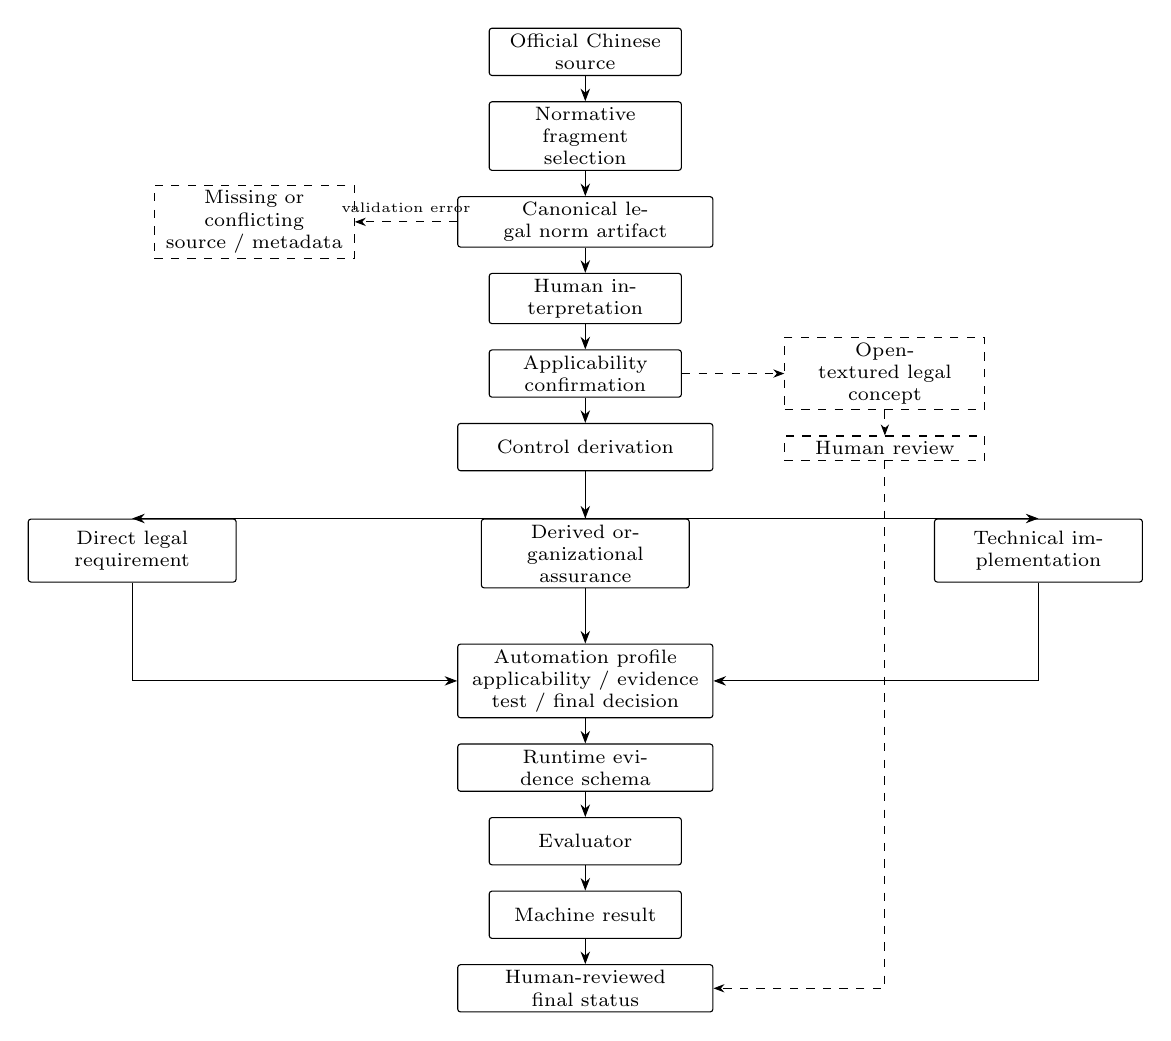
\begin{tikzpicture}[
  font=\scriptsize,
  node distance=3.2mm and 5.5mm,
  box/.style={draw, rounded corners=1pt, align=center, minimum height=6mm, text width=23mm, inner sep=2pt},
  wide/.style={box, text width=31mm},
  branch/.style={box, text width=25mm, minimum height=8mm},
  route/.style={draw, dashed, align=center, text width=24mm, inner sep=2pt},
  flow/.style={-{Stealth[length=1.6mm]}, line width=.35pt},
  review/.style={-{Stealth[length=1.4mm]}, dashed, line width=.35pt}
]
  \node[box] (source) {Official Chinese\\source};
  \node[box, below=of source] (fragment) {Normative fragment\\selection};
  \node[wide, below=of fragment] (norm) {Canonical legal norm artifact};
  \node[box, below=of norm] (interpretation) {Human interpretation};
  \node[box, below=of interpretation] (applicability) {Applicability\\confirmation};
  \node[wide, below=of applicability] (derivation) {Control derivation};

  \node[branch, below left=6mm and 28mm of derivation] (direct) {Direct legal\\requirement};
  \node[branch, below=6mm of derivation] (derived) {Derived organizational\\assurance};
  \node[branch, below right=6mm and 28mm of derivation] (technical) {Technical implementation};
  \node[wide, below=7mm of derived] (profile) {Automation profile\\applicability / evidence test / final decision};
  \node[wide, below=of profile] (runtime) {Runtime evidence schema};
  \node[box, below=of runtime] (evaluator) {Evaluator};
  \node[box, below=of evaluator] (machine) {Machine result};
  \node[wide, below=of machine] (final) {Human-reviewed final status};

  \node[route, left=13mm of norm] (validation) {Missing or conflicting\\source / metadata};
  \node[route, right=13mm of applicability] (open) {Open-textured legal\\concept};
  \node[route, below=of open] (human) {Human review};

  \draw[flow] (source) -- (fragment);
  \draw[flow] (fragment) -- (norm);
  \draw[flow] (norm) -- (interpretation);
  \draw[flow] (interpretation) -- (applicability);
  \draw[flow] (applicability) -- (derivation);
  \draw[flow] (derivation.south) |- (direct.north);
  \draw[flow] (derivation) -- (derived);
  \draw[flow] (derivation.south) |- (technical.north);
  \draw[flow] (direct.south) |- (profile.west);
  \draw[flow] (derived) -- (profile);
  \draw[flow] (technical.south) |- (profile.east);
  \draw[flow] (profile) -- (runtime);
  \draw[flow] (runtime) -- (evaluator);
  \draw[flow] (evaluator) -- (machine);
  \draw[flow] (machine) -- (final);
  \draw[review] (norm.west) -- (validation.east) node[midway, above, font=\tiny] {validation error};
  \draw[review] (applicability.east) -- (open.west);
  \draw[review] (open) -- (human);
  \draw[review] (human.south) |- (final.east);
\end{tikzpicture}
}
\caption{Traceable transformation pipeline from a formal Chinese legal provision to a machine-readable control and reviewed evaluation result.}
\label{fig:transformation-pipeline}
\end{figure*}

Each selected clause is decomposed using an annotation protocol. The required fields include formal Chinese source text, working English translation, official source URL, source document, article number, normative fragment, regulated actor, modality, action, object, trigger, exception, timing, required evidence, control objective, test logic, automation level, ambiguity level, review note, source effective date, author review status, legal expert review status, and interpretation version. This keeps document-level structure, legal semantics, and executable tests distinct rather than treating a markup format as a complete legal interpretation \cite{akomaNtoso2018,legalRuleMl2021}.

The protocol treats the Chinese source text as authoritative for the research artifact. English text is recorded only as a working translation. The schema no longer labels an English summary as original text. This distinction matters because a control should remain traceable to the formal legal source rather than to an informal summary.

The semantic record preserves source and article; normative fragment; regulated actor, action, and object; trigger, exception, and timing; evidence requirement; test logic; automation and ambiguity level; and author-versus-expert review status. These fields preserve both the legal relation and the boundary of the engineering interpretation.

\section{Machine-Readable Schema}

The repository contains two schemas. The legal norm schema represents the human-reviewed interpretation of a clause. The control schema represents the executable control derived from that norm. Both require source traceability, evidence requirements, test logic, automation level, and review status. The source block includes Chinese title, English title, issuing authority, article, formal Chinese source text, working English translation, official source URL, promulgation date, effective date, and retrieval date.

\begin{lstlisting}
norm_id: CN-AIGC-LABEL-001

applicability:
  human_confirmed_fields:
    - output_matches_explicit_label_scenario

automation_profile:
  applicability: human_confirmed
  evidence_test: fully_automatable
  final_decision: automated_after_confirmation

test:
  expression: visible_label_present == true

review:
  legal_expert_review_status: not_reviewed
\end{lstlisting}

The schema is intentionally modest. It does not encode all legal meaning. It checks whether a proposed rule contains the minimum information needed for traceability and execution. The separation of legal norm, machine-readable control, and assessment artifact is informed by machine-readable control approaches such as OSCAL \cite{nistOscal} and legal-rule representation approaches such as LegalRuleML \cite{legalRuleMl2021}. Source metadata validation checks that required source fields are present and internally consistent; it does not automatically prove that the stored text remains identical to the current official webpage. The prototype therefore records \texttt{metadata\_only} source-snapshot status unless independent snapshot or manual verification is recorded.

\subsection{Runtime Evidence Schema}

The repository separates four artifacts in the execution path:

\begin{lstlisting}
Norm schema
-> Control schema
-> Runtime evidence schema
-> Evaluation result
\end{lstlisting}

The norm artifact records a human-reviewed legal interpretation; the control schema records the machine-readable rule derived from it; and the runtime evidence schema validates the shape of business facts, human confirmations, and keyed human-review records supplied to the evaluator. Runtime schema validation is intentionally generic for business facts because fields differ by control, but it strictly validates confirmation and review records. Semantic evaluation remains separate: it checks whether a confirmation agrees with business evidence and whether a required review key is complete.

\subsection{Source Excerpt Integrity}

Each norm stores a SHA-256 digest of the normalized Chinese source excerpt, computed from \texttt{source\_text\_zh.strip().encode("utf-8")}. The digest detects a change to the repository artifact. It does not establish that the stored excerpt is identical to the current official webpage; that question remains subject to independent source verification. The \texttt{metadata\_only} status and excerpt integrity are therefore distinct claims. This boundary is important because formal structure can support review without resolving the interpretive uncertainty of legal language \cite{mohun2020cracking,sergot1986nationality}.

\section{Human Review and Traceability}

The framework does not assume that machine-readable representations are machine-interpreted. The machine executes a reviewed representation. Human review remains necessary for selecting clauses, identifying normative fragments, interpreting ambiguous obligations, determining applicability, and deciding whether evidence is legally sufficient.

The initial interpretation in this prototype is performed by the author as a research exercise. The repository therefore separates \texttt{author\_review\_status} from \texttt{legal\_expert\_review\_status}. A status of ``reviewed'' currently means internally reviewed by the researcher unless a qualified legal expert review is separately recorded. Expert review is especially important for public-opinion or social-mobilization capacity, sensitive personal information classification, label prominence, and obligations that use open-textured terms such as effective measures.

Rules are classified into three automation levels. Metadata field presence may be fully automatable once applicability is established. Human-confirmed applicability is represented as a structured record that identifies the confirmed value, reviewer role, and review time, and is checked against business evidence by the evaluator. Label prominence, confusion risk, and content-safety adequacy are routed through a declared human-review key because legal adequacy cannot be reduced to a single Boolean field.

\subsection{Multi-Layer Automation Profile}

A single automation label can conceal an important distinction: a control may have a deterministic evidence test while its legal applicability remains human-confirmed or its final conclusion requires review. The framework therefore records applicability automation, evidence-test automation, and final-decision automation separately; the complete inventory appears in Table~\ref{tab:all-automation-profiles}.

\subsection{Direct Obligations and Derived Organizational Controls}

The framework distinguishes a direct legal obligation from a supporting organizational assurance control. The first maps the legal duty itself into a machine-readable test. The second records an evidence practice that an engineering organization may choose in order to support assurance. For Deep Synthesis Article 14, the direct control checks that the provider presents a user prompt concerning notice and separate consent. A separate derived control checks whether edited-person consent evidence and scope review have been retained. The latter is not presented as a verbatim statutory requirement that a provider must retain a particular record in every case. Each control records \texttt{control\_derivation\_type} and \texttt{control\_component} to make this relationship visible.

\subsection{Lifecycle Scope}

The Article 9 exception in the Labeling Measures is scoped to provider delivery to the requesting user. A pass only means that the prototype found the specified delivery-exception evidence. It does not decide later publication, user declaration, dissemination-platform identification, or platform notice obligations. The prototype deliberately does not automate the complete dissemination chain.

\section{Case Study: Synthetic Actor and Digital Human Rules}

The case study includes controls for visible AIGC label existence, visible-label prominence, metadata labels, GB metadata fields, PIPL separate consent, biometric-like classification, deep-synthesis face/voice user-prompt and consent-assurance controls, model filing applicability, content-safety principles, complaint mechanisms, and deep synthesis confusion-risk labeling. Table~\ref{tab:end-to-end-example} traces one existing visible-label control without adding a new rule or data artifact.

\begin{table}[t]
\caption{End-to-End Transformation Example}
\label{tab:end-to-end-example}
\centering
\footnotesize
\begin{tabularx}{\columnwidth}{@{}p{0.20\columnwidth}X@{}}
\toprule
\textbf{Stage} & \textbf{Representation} \\
\midrule
Source & Labeling Measures, Articles 4 and 9~\cite{aigcLabelingMeasures2025}. \\
Trigger & AI-generated, user-facing content within a human-confirmed explicit-label scenario. \\
Exception & Documented provider-delivery exception; downstream publication remains outside this result. \\
Control & \texttt{CTRL-AIGC-VISIBLE-LABEL-EXISTENCE}. \\
Machine result & Pass when a visible label exists or scoped exception evidence is complete. \\
Final scope & Provider delivery only \\
\bottomrule
\end{tabularx}
\end{table}

The complete automation profiles and aggregate coverage are reported in the Results section.

\section{Results}

The results concern repository-level structural and behavioral validation, not independent legal validation. The analysis for RQ1 yielded 13 core representation elements: source, normative fragment, actor, modality, action, object, trigger, exception, timing, evidence requirement, ambiguity, automation profile, and review status. For RQ2, all 12 controls preserved end-to-end source-to-control traceability in the validated repository state. For RQ3, only the two metadata controls were fully automated across applicability, evidence testing, and final decision; the remaining controls retained a confirmation or review boundary. For RQ4, all 21 designed cases followed their expected routing. Table~\ref{tab:coverage} reports the selected corpus and its derived artifacts. The five instruments are intentionally representative rather than exhaustive. The 12 controls comprise eight direct legal requirements, two derived organizational assurance controls, and two technical implementation controls.

\begin{table}[!t]
\centering
\footnotesize
\caption{Repository Artifact and Control Coverage}
\label{tab:coverage}
\begin{tabular}{@{}lr@{}}
\toprule
\textbf{Artifact} & \textbf{Count} \\
\midrule
Source instruments & 5 \\
Canonical norm artifacts & 11 \\
Machine-readable controls & 12 \\
Direct legal requirement controls & 8 \\
Derived organizational controls & 2 \\
Technical implementation controls & 2 \\
Designed validation cases & 21 \\
\bottomrule
\end{tabular}
\end{table}

Table~\ref{tab:all-automation-profiles} records the complete automation-profile inventory. Two metadata controls have automated applicability, deterministic evidence checks, and automated final results. The remaining controls retain a human confirmation or human-review boundary. Thus RQ3 is not answered with a single automation claim: evidence checking can be deterministic while applicability or the final conclusion remains review-dependent.

\begin{table*}[!t]
\centering
\scriptsize
\caption{Automation Profiles for All Machine-Readable Controls}
\label{tab:all-automation-profiles}
\begin{tabularx}{\textwidth}{@{}p{0.36\textwidth}p{0.20\textwidth}p{0.22\textwidth}p{0.22\textwidth}@{}}
\toprule
\textbf{Control} & \textbf{Applicability} & \textbf{Evidence test} & \textbf{Final decision} \\
\midrule
Visible-label existence & Human-confirmed & Fully automatable & Automated after confirmation \\
Visible-label prominence & Human-confirmed & Partially automatable & Human review required \\
Metadata label & Fully automatable & Fully automatable & Fully automatable \\
GB metadata fields & Fully automatable & Fully automatable & Fully automatable \\
PIPL separate-consent evidence & Human-confirmed & Fully automatable & Human review required \\
PIPL biometric classification & Fully automatable & Partially automatable & Human review required \\
Deep-synthesis face/voice user prompt & Fully automatable & Fully automatable & Human review required \\
Deep-synthesis consent assurance & Fully automatable & Fully automatable & Human review required \\
Model filing & Human-confirmed & Fully automatable & Human review required \\
Content-safety principle & Fully automatable & Partially automatable & Human review required \\
Complaint mechanism & Fully automatable & Fully automatable & Human review required \\
Deep-synthesis confusion-risk label & Human-confirmed & Partially automatable & Human review required \\
\bottomrule
\end{tabularx}
\end{table*}

The validation layers in Table~\ref{tab:validation-results} all completed successfully in the repository state used for this draft. `Pass' means that the relevant structure or expected routing was checked, not that a source interpretation has been independently confirmed as legally correct. A dependency deprecation warning, when emitted by the test environment, is a reproducibility note rather than a substantive result.

\begin{table*}[!t]
\centering
\footnotesize
\caption{Repository Validation Results}
\label{tab:validation-results}
\begin{tabularx}{\textwidth}{@{}p{0.30\textwidth}p{0.16\textwidth}p{0.46\textwidth}@{}}
\toprule
\textbf{Validation layer} & \textbf{Result} & \textbf{Scope} \\
\midrule
Norm schema & Pass & All 11 canonical norm artifacts \\
Control schema & Pass & All 12 controls \\
Cross-file integrity & Pass & Norm, source, mapping, annotation, and traceability artifacts \\
Source-excerpt hash & Pass & Stored excerpt integrity for 11 norms \\
Runtime-evidence schema & Pass & All 21 validation-case inputs \\
Evaluator cases & 21/21 & Expected status routing \\
Pytest & 46 passed & Regression and integrity tests \\
\bottomrule
\end{tabularx}
\end{table*}

Table~\ref{tab:failure-modes} summarizes the designed adverse cases. They address RQ4 by showing that the evaluator can route evidence to \texttt{pass}, \texttt{fail}, \texttt{review}, \texttt{not\_applicable}, or \texttt{validation\_error} according to the declared boundary. In particular, a normal Boolean is not treated as a human confirmation, a complete Article 9 record passes only within provider delivery, and an aggregate metadata flag cannot mask an absent required field.

\begin{table*}[!t]
\centering
\footnotesize
\caption{Failure-Mode Validation}
\label{tab:failure-modes}
\begin{tabularx}{\textwidth}{@{}p{0.45\textwidth}p{0.24\textwidth}p{0.23\textwidth}@{}}
\toprule
\textbf{Failure mode} & \textbf{Expected routing} & \textbf{Observed routing} \\
\midrule
Missing human confirmation & Review & Review \\
Human-confirmation value conflict & Review & Review \\
Article 9 exception fields present but conditions unsatisfied & Fail & Fail \\
Invalid runtime evidence & Validation error & Validation error \\
Missing or orphan norm & Validator error & Validator error \\
Source-excerpt hash mismatch & Validator error & Validator error \\
Required human review absent & Review & Review \\
Required metadata field present but null or invalid & Fail & Fail \\
\bottomrule
\end{tabularx}
\end{table*}

These outcomes establish control-to-norm traceability for all controls in the selected repository corpus and demonstrate the intended automation boundary. They do not establish the correctness of the legal mapping, external validity in a real service, or legal compliance of any organization. The previous 1,000-request synthetic pipeline remains a supplementary proof of concept: it exercises structured controls against synthetic operational records but is not the central result of this paper.

\section{Independent Review Design}

No independent reviewer has yet evaluated the corpus. The repository therefore provides a planned, rather than completed, independent-review protocol and blank templates for second-coder review, legal-expert review, and adjudication. Because the corpus contains only 11 norms, the planned second coder reviews all 11 directly from the formal Chinese source before seeing the author's decomposition. The coding fields are source article, normative fragment, actor, modality, action, object, trigger, exception, timing, ambiguity, automation profile, control derivation type, and required evidence fields.

The proposed design requires a 100\% source-and-article match. It uses exact agreement for categorical fields, Cohen's kappa for modality, automation, and derivation type, and Jaccard similarity for trigger, exception, and evidence-field sets. A target exact agreement of at least 80\% for other structured fields is a planned decision rule, not a current result. Krippendorff's alpha may be reported only with a caution that 11 norms provide an unstable estimate. All disagreements retain both original codings and are logged as \texttt{accepted\_author}, \texttt{accepted\_reviewer}, \texttt{revised\_by\_consensus}, \texttt{needs\_legal\_expert\_review}, or \texttt{disputed}.

A future qualified legal reviewer should verify source text and article references; assess whether direct requirements are faithful and derived controls are explicitly labelled; examine Article 9 scope, Article 14 prompt and retention boundaries, filing applicability, biometric classification, open-textured concepts, and material effects of working translations. This future stage is necessary because structured internal consistency does not establish substantive legal validity \cite{legalRuleMl2021,mohun2020cracking}.

\section{Discussion}

The results support four methodological points. First, legal applicability, evidence-test execution, and final decision should be modeled separately. A fully automatable field-presence check does not decide whether a legal trigger has been established or whether a qualitative requirement is adequate. Second, direct legal requirements and derived organizational controls must be distinguishable. Organizations may adopt a stronger evidence-retention practice, but a research artifact should not present it as a verbatim statutory command. Third, machine-readable structure supports repeatability and traceability; it does not allow software to resolve open texture, factual context, or competing interpretations. Fourth, source-excerpt hashes guard the integrity of repository text but do not prove the continuing authenticity or currency of an official source.

The selected Chinese AIGC rules are particularly instructive because their operational obligations mix field-checkable conditions with open-ended concepts such as prominent notice, effective measures, public-opinion or social-mobilization capacity, and adequacy of safety handling. The framework intentionally leaves those boundaries reviewable. It could be extended to more instruments, but this paper prioritizes a small corpus whose provenance and transformation steps can be inspected before expanding scope.

\section{Limitations}

The corpus is small and illustrative, containing 11 norms selected from five instruments. The initial interpretation was completed by one author; no second-coder or qualified legal-expert review has been completed. Working translations are not official translations. Validation cases are designed cases rather than observations of real services. The schema is not a legal ontology, and the evaluator is not a production legal-judgment system. Automation classifications are research judgments that require legal review before operational use. Source hashes establish repository-excerpt integrity, not identity with a current official webpage. Regulations and regulatory interpretations may change. The project uses no real personal, biometric, face, voice, contract, company, customer, or production-media data. It does not certify compliance with any law or standard.

\section{Conclusion}

This paper presents a traceable method for transforming selected Chinese AIGC legal provisions into machine-readable controls. The repository demonstrates that a small corpus can be represented as canonical norms, scoped controls, structured runtime evidence, and review-routed results. Deterministic evidence checks can be automated, while applicability and final legal conclusions remain human-confirmed or human-reviewed where the source requires judgment. The completed validation concerns schemas, traceability, integrity, and designed routing rather than legal correctness or certification. The next research stage is independent coding and qualified legal-expert review, followed by transparent adjudication of unresolved interpretations.

\balance
\bibliographystyle{IEEEtran}
\bibliography{references}

\end{document}
